\documentclass[tikz, border=2pt]{standalone}
\usepackage{tikz}
\usetikzlibrary{arrows.meta}
\begin{document}
    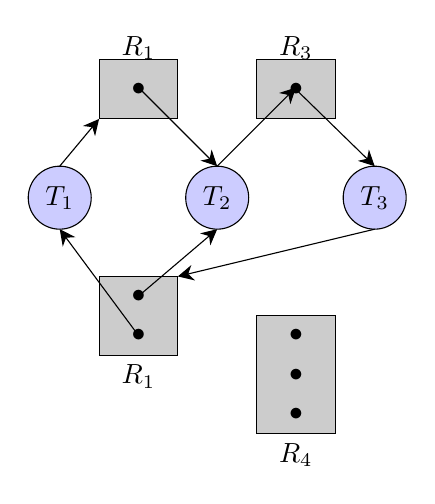
\begin{tikzpicture}
        \draw[fill=black!20] (2,0) rectangle ++(1,1.5) node [midway, below, yshift=-0.75cm] {$R_4$}
            % draw 3 dots top to bottom
            node at (2.5,1.25) {$\bullet$}
            node at (2.5,0.75) {$\bullet$}
            node at (2.5,0.25) {$\bullet$};
        \draw[fill=black!20] (0,1) rectangle ++(1,1) node [midway, below, yshift=-0.5cm] {$R_1$}
            % draw 3 dots top to bottom
            node at (0.5,1.75) {$\bullet$}
            node at (0.5,1.25) {$\bullet$};
        \draw[fill=black!20] (2,4) rectangle ++(1,0.75) node [midway, above, yshift=0.25cm] {$R_3$}
            % draw dot
            node at (2.5,4.375) {$\bullet$};
        \draw[fill=black!20] (0,4) rectangle ++(1,0.75) node [midway, above, yshift=0.25cm] {$R_1$}
            % draw dot
            node at (0.5,4.375) {$\bullet$};
        % \foreach \x in {1,...,3}
            % draw 3 circles between (2,0) and (0,0)
        \draw[fill=blue!20] (-0.5,3) circle (0.4) node {$T_1$};
        \draw[fill=blue!20] (1.5,3) circle (0.4) node {$T_2$};
        \draw[fill=blue!20] (3.5,3) circle (0.4) node {$T_3$};
        \draw[-{Stealth[length=2mm, width=2mm]}] (0.5,1.25) -- (-0.5,2.6);
        \draw[-{Stealth[length=2mm, width=2mm]}] (2.5,4.375) -- (3.5,3.4);
        \draw[-{Stealth[length=2mm, width=2mm]}] (-0.5,3.4) -- (0,4);
        \draw[-{Stealth[length=2mm, width=2mm]}] (0.5,1.75) -- (1.5,2.6);
        \draw[-{Stealth[length=2mm, width=2mm]}] (0.5,4.4) -- (1.5,3.4);
        \draw[-{Stealth[length=2mm, width=2mm]}] (1.5,3.4) -- (2.5,4.4);
        \draw[-{Stealth[length=2mm, width=2mm]}] (3.5,2.6) -- (1,2);
    \end{tikzpicture}
\end{document}